%**************************************************************
% Lab 07: Bit Pattern Detector
%**************************************************************
\chapter{Bit Pattern Detector}

\section{Purpose}

This lab builds a circuit that detects a specific pattern of bits on an input stream. This is a very simple circuit that introduces shift registers. three starter versions of this lab are provided as an iterative process.

\section{Procedure}

\subsection{Subcircuit V1}

Start a new \textit{Logisim-evolution} project and create a subcircuit labeled \lstinline|V1|.

Place a Shift Register (\textit{Memory} library) on the drawing canvas. Set the properties of the shift register to one data bit and four stages. Wire Buttons (\textit{Input/Output} library) to the \textit{R} and \textit{clk} inputs and label those buttons \textit{\texttt{Reset}} and \textit{\texttt{clk}}. Wire a one-bit input pin to the \textit{1,3D} input on the shift register and label it \textit{\texttt{InData}}.

Using a splitter, gather all four outputs into a single bus and wire that bus to one input on a comparator (\textit{Arithmetic} library). Wire a Constant (\textit{Wiring} library) \textit{a} on the other comparator input. Finally, wire a Probe (\textit{Wiring} library) with a Radix set to Hexadecimal to the output bus.

When completed, the circuit should look like Figure \ref{fig:07-01}.

\begin{figure}[H]
	\centering
	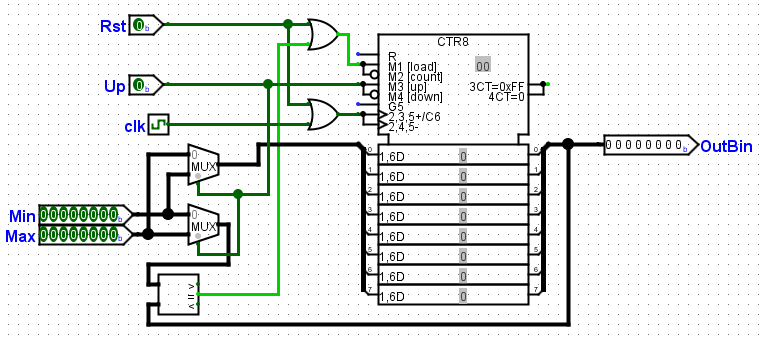
\includegraphics[width=\maxwidth{.95\linewidth}]{gfx/07-01}
	\caption{Pattern Detector, V1}
	\label{fig:07-01}
\end{figure}

\subsection{Testing the Circuit}

\begin{enumerate}
	\item Poke \textit{Reset} to reset the shift register.
	\item Poke \textit{InData} to make it go high and then poke \textit{clk}.
	\item Poke \textit{InData} to make it go low and then poke \textit{clk}.
	\item Poke \textit{InData} to make it go high and then poke \textit{clk}.
	\item Poke \textit{InData} to make it go low and then poke \textit{clk}.
	\item \textit{Detected} should go high.
\end{enumerate}


\section{Challenge}

Whatever

\section{Deliverable}

To receive a grade for this lab, complete the Challenge. Be sure the standard identifying information is at the top left of the \lstinline{main} circuit: 

\bigskip
% The minipage environment keeps the three lines together - no page break.
\begin{minipage}{\linewidth}
	\begin{verbatim}
	George Self
	Lab 07: Bit Pattern Detector
	March 11, 2018
	\end{verbatim}
\end{minipage}
\bigskip

Save the file with this name: \textit{Lab07\_Detect} and submit that file for grading.

